\documentclass[conference]{IEEEtran}

\usepackage[utf8]{inputenc}
\usepackage[T1]{fontenc}
\usepackage{silence}\WarningsOff[latexfont]

\usepackage{amsmath}

\usepackage{graphicx}
\usepackage{cite}
\usepackage{url}
\usepackage[caption=false,font=footnotesize]{subfig}
\usepackage[binary-units,per-mode=symbol]{siunitx}
\sisetup{list-final-separator = {, and }}
\usepackage{booktabs}
\usepackage{pifont}
\usepackage{microtype}
\usepackage{textcomp}
\usepackage[american]{babel}
\usepackage[noabbrev,capitalise]{cleveref}
\usepackage{xspace}
\usepackage{hyphenat}
\usepackage[draft,inline,nomargin,index]{fixme}
\fxsetup{theme=color}
\usepackage{grffile}
\usepackage{xfrac}
\usepackage{multirow}
\RequirePackage{xstring}
\RequirePackage{xparse}
\RequirePackage[index=true]{acro}

\NewDocumentCommand\acrodef{mO{#1}mG{}}{\DeclareAcronym{#1}{short={#2}, long={#3}, #4}}
\NewDocumentCommand\acused{m}{\acuse{#1}}

\usepackage{upquote}

\acrodef{ReLU}{Rectified Linear Unit}

\begin{document}

\title{Assignment 3 - Deep Networks}
\author{
	\IEEEauthorblockN{Davide Pedranz (189295)}
	\texttt{davide.pedranz@studenti.unitn.it}
}

\maketitle

\begin{abstract}
Deep Networks are state of the art techniques for many difficult problems in Machine Learning, widely used for many different tasks, from image recognition to machine translation.
In this assignment, we will use TensorFlow\textsuperscript{TM} to construct and train Deep Networks with different architectures to recognize the handwritten digits of the MNIST dataset.
\end{abstract}

\acresetall

\section{Introduction}
\label{sec:introduction}

Neural Network is a powerful learning algorithm widely used in Machine Learning to solve complex tasks like handwritten text recognition, computer vision, speech recognition and machine translation.
Indeed, Neural Networks are able to represent very complex functions, which make them very adaptable to many different problem.

Depending on the specific task to solve, Neural Networks with different structures can be built and trained.
In this assignment, we will start from the architecture suggested in the TensorFlow\textsuperscript{TM} tutorial \textit{Deep MNIST for Experts} \footnote{\url{https://www.tensorflow.org/versions/master/tutorials/mnist/pros/}} to recognize the handwritten digits of the MNIST \footnote{The MNIST dataset is available at: \url{http://yann.lecun.com/exdb/mnist/}} dataset, then remove one layer at a time and study the behaviour of the new network.
We will explain the structure of each network and the function of each layer.
Finally, we will compare the performances of the different networks.

There are many different libraries available to construct and train Neural Networks.
In this assignment, we will use TensorFlow\textsuperscript{TM}, an open source library for numerical computation using data flow graphs.
It allows to easily define the structure of a Neural Network and efficiently train it.
It was originally developed by the Google Brain Team and is now widely used by many students, researches and companies across the world.

\section{Neural Networks}
\label{sec:nn}

The building block of each Neural Network is the perceptron.
A perceptron is a unit of computation that takes many inputs and compute an output, which is usually the result of the application of some activation function to the weighted sum of the inputs.
In other words, a perceptron computes the dot product between the inputs and some learned weights, i.e.\ it measures the similarity between the input and some internal representation.

Perceptron are organized in layers, which in turn form a network.
Each network can have a different number of layers and each layer can have a different number of perceptrons.
Some of the main types of layers include ``Fully Connected'', ``Softmax'', ``Convolutional'' and ``Pooling''.

In the following sections, we will examine how this layers are build and what is their function in a Deep Network for handwritten digits recognition.

\section{Fully Connected Layer}
\label{sec:fc_layer}

In a Fully Connected Layer each perceptron is connected to each of the outputs of the previous layer.
Both the inputs and the outputs are organized as a one dimensional array.

The output of each perceptron is computed as an activation function of the weighted sum of all the inputs plus a bias.
The activation function aims to break the linearity of perceptron, allowing the successive layers to build increasingly complex non-linear features of the original input.
Common choices for the activation are the Sigmoid and the \ac{ReLU} function.

The Sigmoid function as the form:
\begin{equation*}
    f(x) = \frac{1}{1 + e^{-x}}
\end{equation*}
and can be seen in \cref{fig:sigmoid}.
It has the nice property that it is almost linear and quite steep in an interval of zero, which makes the learning process very quick.
On the other side, is saturates very quickly as soon as the input moves away from zero.
This can accidentally ``kill'' the perceptron, since the backpropagation algorithm multiplies the error from the following layer to the local gradient to calculate the weights update \cite{CS231n}.

\begin{figure}[ht]
	\centering
	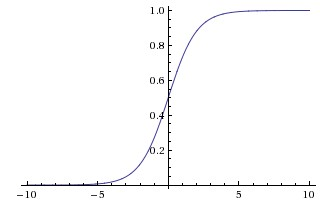
\includegraphics[scale=0.6]{figures/sigmoid}
	\caption{The Sigmoid function.}
	\label{fig:sigmoid}
\end{figure}

A popular alternative is the \ac{ReLU} function.
\ac{ReLU} is defined as follows:

\begin{equation*}
    f(x) = max(0, x)
\end{equation*}

and can be saw in \cref{fig:relu}.

\begin{figure}[ht]
	\centering
	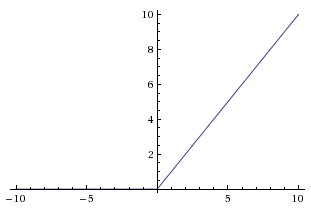
\includegraphics[scale=0.6]{figures/relu}
	\caption{The \ac{ReLU} function.}
	\label{fig:relu}
\end{figure}

\ac{ReLU} has been shown to greatly accelerate the learning process compared to the Sigmoid function \cite{krizhevsky2012imagenet}.
Another advantage is that it does not require to compute complex functions like exponentiation, but simply a threshold.
Unfortunately, \ac{ReLU} units suffer of the same ``dying'' problem of Sigmoid ones.
With high learning rates, the weights of the perceptron can be updated in such a way that its gradient become zero (and will never be updated again).
To reduce this problem, a proper choice the learning rate is necessary \cite{CS231n}.

\section{Softmax}
\label{sec:softmax}

Softmax is a generalization of the Logistic Regression classifier to multiclass problems.
It computes the best class by applying a cross-entropy loss function to a weighted sum of the inputs (dot product of inputs and learned weights).
More formally, it computes an evidence score for each class $i$
\begin{equation*}
    evidence_i = \sum_{j}{W_{ij} x_j + b_i},
\end{equation*}
then it normalizes the scores to a probability distribution over the $i$ possible values
\begin{equation*}
    softmax_i = \frac{e^{evidence_i}}{\sum_{j}{e^{evidence_j}}}.
\end{equation*}

Softmax is commonly used as the last layer of a Deep Network for classification problems.
Please note that in this case the activation function is omitted since an activation value is already computed by the Softmax function.

\section{Convolutional Networks}
\label{sec:conv_net}

In traditional Neural Networks, the input is encoded as a vector of raw numbers which is given as input to the first layer.
This approach does not scale well to images.
Let's consider a 200x200 pixel image with 3 colors.
Each neuron of the first layer will have $200 * 200 * 3 = 120,000$ weights to learn.
And this takes into account only a single neuron in the first layer.
The main problem here is that we do not consider the structure of the input, which is lost during its encoding into a one dimensional array.
In case, for instance, of image recognitions, the actual position of the pixels is very important to understand its meaning.

Convolutional Neural Networks try to exploit the structure of the input to optimize the learning of images with the introduction of Convolutional layers and Pooling layers in addition to traditional Fully Connected ones.
The new types of layer have the scope to extract features from the images, so that the traditional Fully Connected layers can work on meaningful features instead of raw pixel values.
In both Convolutional and Pooling layers, perceptrons are organized in three dimensions: width, height and depth.
Depth refers to different channels of the image representation, for instance RGB for colors.

\section{Convolutional Layer}
\label{sec:conv_layer}

A Convolutional layer consist of a set of learnable filters.
Each filter is spatially small, but extends through the full depth of the input.
The patched is moved on all the image surface and creates a 2-dimensional feature map.
The results of the computation of each filter are then stacked on each other and form the input for the next layer of the network.
The output of each filter is computed, as for normal perceptrons, as the result of an activation function of the dot product of the inputs and the internal learned weights.
It is important to underline that the weights are unique for each filter, which means that the same values are used for each piece of image input for a single filter.
This process can be seen in the \cref{fig:convolution}.

\begin{figure}[ht]
	\centering
	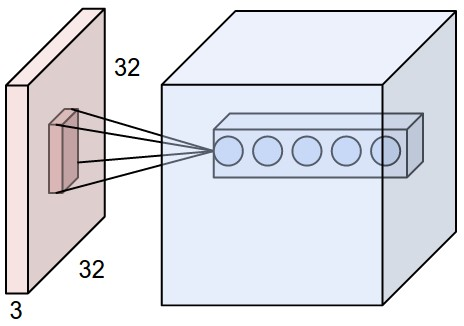
\includegraphics[scale=0.35]{figures/convolution}
	\caption{Illustration\protect\footnotemark ~of the computation of a Convolutional layer. In this example, 5 different filters (in blue) are computed on the original image (in red). Each filter is computed by moving a patch (the small red square) around the input image.}
	\label{fig:convolution}
\end{figure}
\footnotetext{Illustration taken from \url{https://cs231n.github.io/convolutional-networks/}}

A Convolutional layer has some hyperparameters, which determine how the filters are applied to the input.
The main hyperparameters are:
\begin{itemize}
    \item{\textbf{Receptive Field}, which represent the size of the filter. In other words, it determines the dimension of the patch used to compute the filter on the input image. Typical sizes range from 3x3 to 7x7 pixels.
    \item{\textbf{Depth}, which determines the number of filter to be applied. Sometimes this is also called fibre.}
    \item{\textbf{Stride}, which determines the amount of pixel the patch is moved on the image each time. Common values are 1 and 2 pixel.}
}
\end{itemize}

\section{Pooling Layer}
\label{sec:pool_layer}

Convolutional layers can generate outputs that are bigger than the original input by computing a high number of filters.
Pooling layers are commonly inserted in-between successive Convolutional layers to progressively reduce the spatial size of the representation, in order to reduce the amount of parameters and computation in the network.

A Pooling layer re-sizes the input spatially, while it does not change its depth.
As for the case of the Convolutional layer, a patch is moved around the input and some aggregation function is computed to reduce the inputs to a single value.
The most common operator is the max function, even though other operations are possible \cite{CS231n}.

A Pooling layer requires to set some hyperparameters:
\begin{itemize}
    \item{\textbf{Spatial Extent}, which determines the dimension of the patch used to compute the aggregation function on the input image (similarly to the Receptive Field for Convolutional layers).}
    \item{\textbf{Stride}, which determines the amount of pixel the patch is moved on the image each time.}
\end{itemize}
A typical setting is to use max pooling with a spatial extent of 2x2 pixels and stride of 2, as shown in \cref{fig:pooling}.

\begin{figure}[ht]
	\centering
	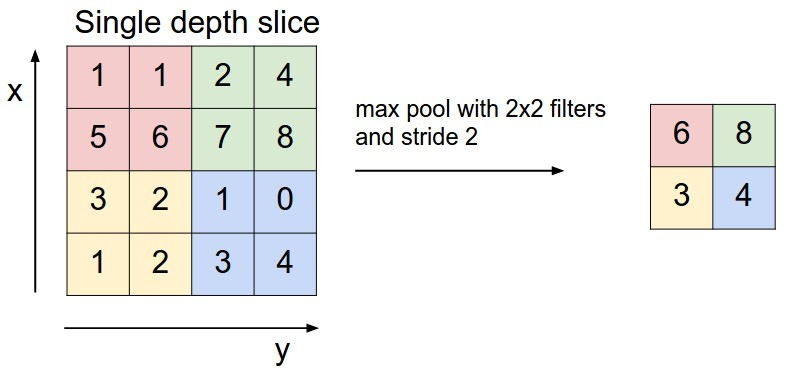
\includegraphics[scale=0.30]{figures/pooling}
	\caption{Illustration\protect\footnotemark ~of the pooling process. In this example, a patch of size 2x2 pixel is moved of 2 pixel at a time. The value computed is the maximum between the current values of the patch.}
	\label{fig:pooling}
\end{figure}
\footnotetext{Illustration taken from  \url{https://cs231n.github.io/convolutional-networks/}}

\section{Dropout}
\label{sec:dropout}

Neural networks, like many other learning algorithms, can suffer from overfitting the data.
A simple technique to avoid overfitting in deep networks is the Dropout.

Dropout is an extremely simple and effective technique recently introduced by Srivastava et al.\ \cite{srivastava2014dropout}.
It consists in randomly turning off perceptrons during the training phase:
at each epoch of training, perceptrons are kept active only with some probability p (a hyperparameter), otherwise they are set to zero.
The process can be see in \cref{fig:dropout}, taken from the original paper.
Dropout is not applied during test and allows to ensemble the different parameters learned by some group of perceptrons during the training.

\begin{figure}[ht]
	\centering
	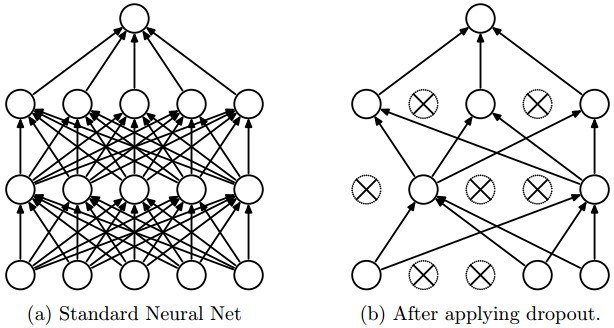
\includegraphics[width=\columnwidth]{figures/dropout}
	\caption{Changes in the neural network after applying Dropout.}
	\label{fig:dropout}
\end{figure}

\section{MNIST Handwritten Digits}
\label{sec:mnist}

The MNIST is a database of handwritten digits.
It is composed by a training set of 60,000 examples and a test set of 10,000 examples, both available on the website of Yann LeCun\footnote{\url{http://yann.lecun.com/exdb/mnist/}}.
The digits have been size-normalized to 20x20 pixel and centered in a fixed-size image of 28x28 pixel.
The images are in black and white, so their depth is equal to 1.

\section{Deep Networks Models}
\label{sec:models}

This section describes and compare the original model proposed by the TensorFlow\textsuperscript{TM} tutorial and three possible modifications.
All network are initialized using the same seed for random number generation in order to obtain results with are comparable.
Also the selection of the initial subsets of the training and test sets are done with the same fixed seed.


\subsection{Original Model}

The original network proposed has the following architecture:
a Convolutional layer, a Pooling layer, another Convolutional layer, another Pooling layer, a Fully Connected layer with \ac{ReLU} activation function and Dropout and a Softmax output layer.
The first Convolutional layer computes 32 filters, while the second one 64.
Both Pooling layers reduces the dimension of the image by applying max pooling with 2x2 pixel patches and stride 2.
\cref{fig:graph} shows the structure of the resulting network.

\begin{figure}[t]
	\centering
	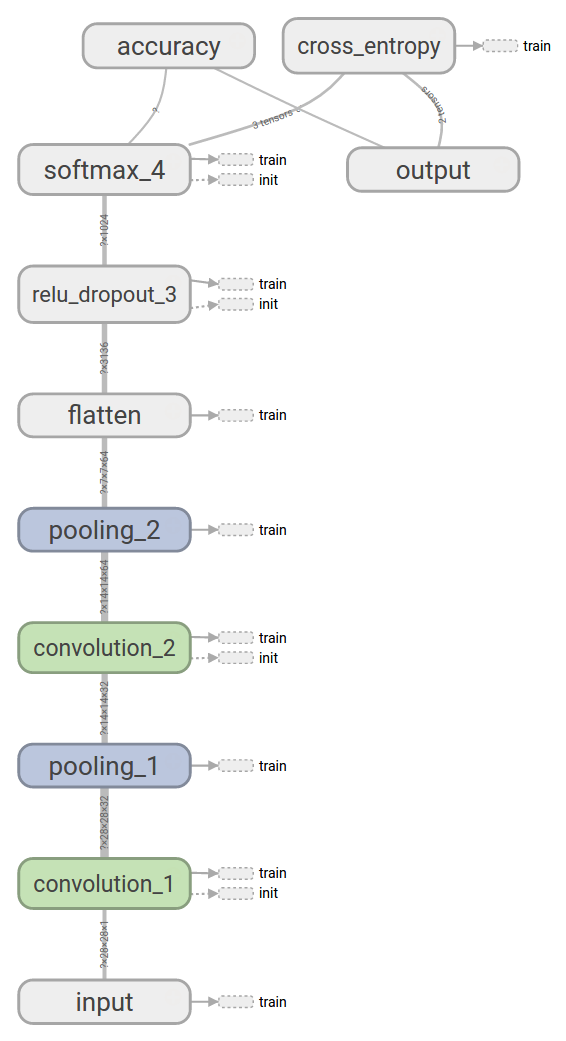
\includegraphics[width=\columnwidth]{figures/graph}
	\caption{Structure of the original Deep Network used for the MNIST handwritten digits recognition, visualized using the TensorBoard tool.}
	\label{fig:graph}
\end{figure}

The Convolutional layers are used to extract features from the images, which are then used by the Fully Connected layer and the Softmax layer to compute the most probable class.
Pooling layers and Dropout are used to prevent the network to overfit the training data.
Note that the image is reshaped into a one dimensional array after the second Pooling layer, in order to be processed by the Fully Connected layer.

At each training step, the network is trained with a batch of 50 images, randomly selected from the train dataset.
The network is trained to minimize the generalized cross entropy function for a multiclass problems.
After 20000 epochs of training, the network has an accuracy of $99.17\%$ on the complete test set.
It is not clear if the accuracy could get better with more training, since its accuracy over time is not stable (see \cref{fig:performances}).

\begin{figure}[t]
	\centering
	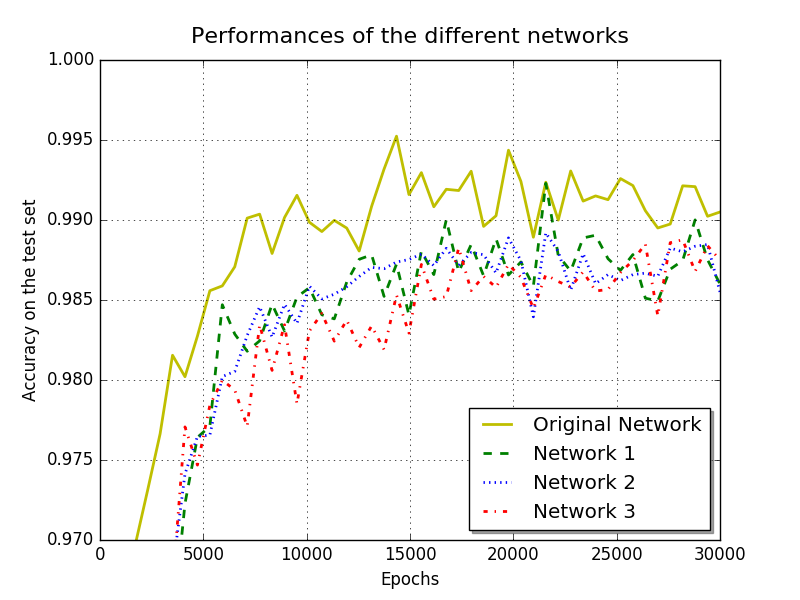
\includegraphics[width=\columnwidth]{figures/performances}
	\caption{The graph shows the performances of the different networks on the test set over epochs of training. The plotted accuracies are measured on a random fixed subset of $1000$ elements of the test set, equal for all the networks.}
	\label{fig:performances}
\end{figure}


\subsection{Model 1}

The first modification to the original model consist in removing the first level of Convolution and Pooling.
The second Convolutional layer is now directly applied to the original image.
The rest of the network and all hyperparameters are unchanged.

The performance of the network is closed to the original one, with an accuracy of $98.99\%$ on the test set.
As for the original model, it is not clear whether the accuracy could increase with more training. 


\subsection{Model 2}

The second modification is very similar to the previous one. Instead of removing the first one, we are removing the second Convolution and Pooling layers.
The resulting network is almost identical to Model 1, but with the difference that the layer is computing 32 filters instead of 64.
The accuracy of this model is $98.94\%$.


\subsection{Model 3}

The third moditifaction consist in removing the Fully Connected layer.
The accuracy of this network is slighly worse then the other models and scores $98.89\%$.
This is probably due to the absence of any fully connected layer that properly combines the features extracted by the convolutional layer.
Like for the other networks, it is not clear if the performances can improve with more training.

\section{Conclusion}
\label{sec:conclusion}

None of the proposed modification achieved to improve the accuracy of the original network.
The results are summarized in table \cref{tab:summary}.
The two layers of convolution were able to extract better features then the single layers of models 1 and 2.
The worse performances of model 3 suggest the need of at least one Fully Connected layer to learn how to combine the features extracted by the previous layers in order to make accurate predicitons.

\begin{table}
	\centering
	\caption{Summary of the performances of the different networks}
	\label{tab:summary}
	\begin{tabular}{lccc}
		\toprule
			\multicolumn{1}{l}{Network} &
			\multicolumn{1}{c}{Accuracy (train)} &
			\multicolumn{1}{c}{Accuracy (test)} \\
		\midrule
			Original & 1.0000 & 0.9917 \\
			Model 1  & 1.0000 & 0.9899 \\
			Model 2  & 0.9962 & 0.9894 \\
			Model 3  & 0.9950 & 0.9888 \\
		\bottomrule
	\end{tabular}
\end{table}


\bibliographystyle{IEEEtran}
\bibliography{references}

\end{document}
